\section{Experimental Evaluation}
\label{sec:experiments}
% We evaluate our certificate synthesis methods on two benchmark systems to demonstrate: the effectiveness of transition certificates for LTL verification; and computational efficiency compared to (neural) closure certificate methods. In the first system, the Kuramoto Oscillator model, which includes 1D and 2D scenarios, we consider the problem of safety verification and convert the safety objective into an LTL specification. We then search for a transition safety certificate over the product of the system and the NBA representing the complement of the LTL specification. In the second system, the two-room temperature model, we consider the problem of persistence verification. To do so, we convert the objective into an LTL specification and simultaneously search for transition safety and transition persistence certificates, thereby demonstrating the complementary advantages of transition certificates. All experiments are run on Ubuntu 22.04.3 LTS (Intel i7-9750H, 8 GB RAM). For the first case, we use dReal (with precision 0.0001) for verification because the system dynamics involves the transcendental function​ $\sin$. For the second system, we use z3 for verification. For polynomial templates, we use z3 to solve a linear programming problem to find candidate certificates. For neural templates, the candidate generation phase employs the Adam optimizer with a learning rate of 0.001 for 1000 iterations to minimize the loss function.


We evaluate the proposed transition certificate synthesis methods on two benchmark systems to demonstrate: their effectiveness in formal LTL verification, and their computational efficiency compared to  (neural) closure certificate methods. For the first benchmark, the Kuramoto Oscillator model (covering both 1D and 2D scenarios), we verify the system against specified LTL properties. For the second benchmark, the two-room temperature model, we demonstrate the versatility of our approach by synthesizing transition certificates to satisfy complex LTL requirements and highlight their complementary advantages in handling diverse temporal specifications. All experiments are conducted on Ubuntu 22.04.3 LTS (Intel i7-9750H, 8 GB RAM). During candidate generation, Z3 addresses the constrained optimization for polynomial templates, whereas neural network templates are trained using the Adam optimizer (learning rate 0.001, 1000 iterations) to minimize the loss function. For formal verification, we employ dReal (precision 0.0001) to handle the transcendental $\sin$ functions in the Kuramoto Oscillator model, while Z3 is utilized for the temperature model. 

\subsection{Kuramoto Oscillator}
\subsubsection{One-Dimensional System}
% 系统介绍
The first benchmark is a Kuramoto oscillator system, formally defined as $\mathfrak{S} = (\mathcal{X}, \mathcal{X}_0, f)$ with dynamics adapted from~\cite{anand2022small}. The system operates within the state space $\mathcal{X} = [0, 2\pi]$, starting from an initial region $\mathcal{X}_0 = [\frac{4\pi}{9}, \frac{5\pi}{9}]$. To evaluate LTL verification, we specify an unsafe region $\mathcal{X}_u = [\frac{7\pi}{9}, \frac{8\pi}{9}]$ within the temporal properties. The discrete-time transition function $f$ is given by:
\begin{align}
f(x) = x + t_s\Omega + t_s K \sin(-x) - 0.532 x^2 + 1.69,
\end{align}
where $x$ represents the oscillator phase. The system parameters are set as follows: sampling time $t_s = 0.1$, natural frequency $\Omega = 0.01$, and coupling strength $K = 0.0006$.



% 如何将安全性验证转化为LTL验证
We consider the LTL specification $\phi = \mathbf{G}\neg a$ over the atomic proposition set $AP = \{a\}$, with the labeling function defined as $\mathfrak{L}(x) = \{a\}$ for $x \in \mathcal{X}_u$ and $\mathfrak{L}(x) = \emptyset$ otherwise. The negated specification, $\neg \phi = \mathbf{F} a$, is characterized by the NBA illustrated in Figure~\ref{pic-tbnba1}. This automaton incorporates accepting transitions $(q_0, \emptyset, q_0)$ and $(q_0, {a}, q_0)$ originating from the initial state $q_0 \in Acc^{\text{start}}$.

\begin{figure}[h]
  \centering
  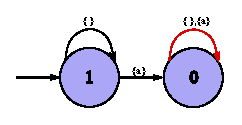
\includegraphics[width=0.3\textwidth]{pic/tbnba1.eps}
  \caption{NBA representing the negated specification $\mathbf{F} a$. Accepting transitions (highlighted in red) are depicted as self-loops at state $q_0$.}
  \label{pic-tbnba1}
\end{figure}

% 多项式模板方法
Based on the definition of transition safety certificates, we implement a polynomial-based CEGIS framework to synthesize certificates that guarantee the satisfaction of the specified LTL property. The polynomial template is structured as follows:
\[
B_0(x, q; \mathbf{c}) = \sum_{i=0}^{4} c_i x^i + \sum_{j=1}^{3} c_{4+j} q^j + c_8 xq.
\]
The synthesis process begins by collecting 30 samples from region $D_0$, 600 from $D_u$, and 1200 from $D_{\mathcal{X}}$. The candidate generation phase is formulated as a constraint satisfaction problem and solved using the Z3 solver. Given that the system dynamics involve the transcendental $\sin$ function, which lies beyond the decision procedures of Z3, we employ the dReal solver during the verification phase to identify counterexamples. The complete CEGIS loop converges in 3.6 seconds, successfully yielding a valid transition certificate:
\[
B_0(x, q) = -1 + 2q^2 - \frac{7}{16}xq.
\]

% 神经模板方法
In addition to polynomial templates, we synthesize a neural transition certificate $B_0(x, q; \theta)$ using the CEGIS framework. The certificate is parameterized by a feedforward neural network with a 2-10-1 architecture, featuring two input nodes for the pair $(x, q)$, a hidden layer of 10 neurons with ReLU activation, and a single linear output. The training process is initialized with a dataset of 250 samples (40 from $D_0$, 70 from $D_u$, and 140 from $D_{\mathcal{X}}$). During each iteration, the dReal solver is employed to identify any points violating the certificate conditions. These identified counterexamples are then incorporated into the training set to progressively refine the candidate certificate. The complete CEGIS loop converges in 3.2 seconds. The valid certificates obtained during the process are provided in the appendix.

\subsubsection{Two-Dimensional System}

The benchmark is further extended to a two-dimensional scenario with state space $\mathcal{X} = [0, \frac{8\pi}{9}]^2$ and initial region $\mathcal{X}_0 = [0, \frac{\pi}{9}]^2$. In this case, the unsafe region $\mathcal{X}_u$ is defined as the boundary corridors of the state space:
\begin{equation}
\mathcal{X}_u = \left([0, \tfrac{8\pi}{9}] \times [\tfrac{5\pi}{6}, \tfrac{8\pi}{9}]\right) \cup \left([\tfrac{5\pi}{6}, \tfrac{8\pi}{9}] \times [0, \tfrac{8\pi}{9}]\right).
\end{equation}
The coupled system dynamics $f$ are governed by:
\begin{equation}
f(x_1, x_2) =
\begin{bmatrix} x_1 \\ x_2 \end{bmatrix}
+ t_s
\begin{bmatrix} \Omega + 1.69 \\ \Omega + 1.69 \end{bmatrix}
+ K t_s
\begin{bmatrix} \sin(x_2 - x_1) \\ \sin(x_1 - x_2) \end{bmatrix}
- 0.532 t_s
\begin{bmatrix} x_1^2 \\ x_2^2 \end{bmatrix}.
\end{equation}
To maintain consistency with the 1D analysis, we define the labeling function such that $\mathfrak{L}(x_1, x_2) = \{a\}$ if $(x_1, x_2) \in \mathcal{X}_u$ and $\emptyset$ otherwise. The verification is performed against the same LTL specification $\phi = \mathbf{G}\neg a$ using the NBA illustrated in Figure~\ref{pic-tbnba1}.


For the two-dimensional system, we first employ a polynomial template $B_0(x_1, x_2, q; \mathbf{c})$. The synthesis process utilizes a dataset of 30 samples from $D_0$, 729 from $D_u$, and 1,458 from $D_{\mathcal{X}}$. Within 7.3 seconds, the CEGIS loop yields a valid transition certificate:
\begin{equation}
B_0(x_1, x_2, q) = -1 + \tfrac{1}{8}x_1 x_2 + \tfrac{3}{2}q^2 - \tfrac{3}{32}q x_1^2 - \tfrac{153}{512}x_2 q.
\end{equation}
Furthermore, we implement a neural network template with a 3-15-1 architecture, featuring three input nodes for the tuple $(x_1, x_2, q)$ and a hidden layer of 15 neurons with ReLU activation. To demonstrate the efficiency of our framework, we initialize the training with a set of points: 40 from $D_0$, 90 from $D_u$, and 180 from $D_{\mathcal{X}}$. The CEGIS loop converges in 234.1 seconds, successfully producing a valid neural certificate in appendix.


\subsection{Two-Room Temperature}

The second benchmark focuses on the formal verification of an interconnected temperature control system, denoted by $\mathfrak{S} = (\mathcal{X}, \mathcal{X}_0, f)$, with its dynamical model adapted from~\cite{anand2024compositional}. The system operates within a state space $\mathcal{X} = [20, 34]^2$, originating from the initial configuration $\mathcal{X}_0 = [21, 24]^2$. The underlying LTL specification pertains to the target region $\mathcal{X}_{VF} = [20, 26]^2$. Specifically, the evolution of the system state is governed by the following discrete-time dynamics $f$:
\begin{equation}
f(x_1, x_2) = 
\begin{bmatrix} 1 - 2\alpha - \theta - \mu u(x_1) & \alpha \\ \alpha & 1 - 2\alpha - \theta - \mu u(x_2) \end{bmatrix}
\begin{bmatrix} x_1 \\ x_2 \end{bmatrix}
+ \mu T_h
\begin{bmatrix} u(x_1) \\ u(x_2) \end{bmatrix}
+ \theta
\begin{bmatrix} T_e \\ T_e \end{bmatrix},
\end{equation}
where the constant parameters are assigned as $\alpha = 0.004$, $\theta = 0.01$, $\mu = 0.15$, $T_h = 40$, and $T_e = 0$. The state-dependent control term is defined as $u(x_i) = 0.59 - 0.011 x_i$ for $i \in \{1, 2\}$.



Consider the set of atomic propositions $AP = \{a, b\}$, where the labeling function is defined as $\mathfrak{L}(x_1, x_2) = \{a\}$ for $(x_1, x_2) \in \mathcal{X}_0$, and $b \in \mathfrak{L}(x_1, x_2)$ for $(x_1, x_2) \in \mathcal{X}_{VF}$. The system is required to satisfy the LTL specification $\varphi = a \Rightarrow \mathbf{FG}\neg b$. The corresponding NBA, which captures the negation of the specification (i.e., $\neg \varphi = a \land \mathbf{GF} b$), is illustrated in Figure~\ref{pic-tbnba2}. To demonstrate the complementary roles of transition safety certificates and transition persistence certificates, we synthesize both types of certificates for this benchmark.


\begin{figure}[h]
  \centering
  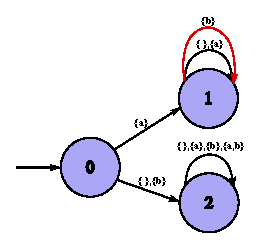
\includegraphics[width=0.3\textwidth]{pic/tbnba2.eps}
  \caption{NBA for $a \land \mathbf{GF} b$ (negation of $a \Rightarrow \mathbf{FG}\neg b$). Accepting transitions (red) are $(q_1, \{b\}, q_1)$ and $(q_1, \{a,b\}, q_1)$.}
  \label{pic-tbnba2}
\end{figure}

Consider the transition safety certificate template and transition persistence certificate template(seen in Appendix~\ref{appendix-experiment}). We simultaneously synthesize them. For the transition safety certificate, we collect 16 samples for $D_0$, 196 for $D_u$, 588 for $D_{\mathcal{X}}$. For the transition persistence certificate, we collect 16 samples for $D_0$ and 196 for $D_{\mathcal{X}}$. We obtain a valid transition persistence certificate $$B_{1,1}(x_1, x_2) = 27 I_{[20,26]^2}(x_1, x_2) - x_1 I_{[20,26]^2}(x_1, x_2)$$ and $\epsilon = 0.25$ in 8.8 seconds.

We synthesize the transition safety certificate $B_1(x_1, x_2, q)$ for $q_1$ and the transition persistence certificate $B_{1,1}(x_1, x_2)$ for $Acc^{1,1}$. We synthesize $B_1(x_1, x_2, q)$ using the CEGIS with neural network template of architecture 3-10-1 (3 inputs for $(x_1, x_2, q)$, 10 hidden neurons with ReLU activation, 1 output). We synthesize $B_{1,1}(x_1, x_2)$ using the CEGIS with neural network template of architecture 2-3-1 (2 inputs for $(x_1, x_2)$, 3 hidden neurons with squared activation, 1 output). For the transition persistence certificate, we collect 100 samples for $D_{\mathcal{X}}$. For the transition safety certificate, we collect 4 samples for $D_0$, 9 for $D_u$, 18 for $D_{\mathcal{X}}$. The entire CEGIS loop terminates in 1228.3 seconds and the valid certificates obtained are provided in the appendix.. 

\subsection{Comparison}
We primarily compare our approach with closure certificates~\cite{murali2024closure} and neural closure certificates~\cite{nadali2024neural}, as they represent recent developments in abstraction-free LTL verification. While the state-triplet method~\cite{wongpiromsarn2015automata} is a foundational approach, it is omitted from our quantitative comparison for two reasons: (1) its inherent conservatism often fails to find valid certificates for complex LTL specifications, particularly those involving persistence properties; and (2) closure certificates~\cite{murali2024closure} were specifically developed to provide more general verification conditions than the state-triplet method. The core idea of closure certificates lies in characterizing an over-approximation of the transition closure, so closure certificates for LTL verification are defined over $\mathcal{X} \times \mathcal{X} \times Q \times Q$. In contrast, our method employs transition safety certificates to directly filter out unreachable automaton states or uses transition persistence certificates to prove that the accepting transitions occur finitely often, so the search space of transition certificates is at most $\mathcal{X} \times Q \times Q$. This allows us to reduce the search space from $\mathcal{X} \times \mathcal{X} \times Q \times Q$ to $\mathcal{X} \times Q \times Q$ and improves synthesis efficiency. For neural templates, we adopt the CEGIS framework, whereas the neural closure certificate approach relies on sampling and posteriori verification: after sampling the state space with a given density $\epsilon$ and safety margin $\eta$, the method trains until the loss converges to zero and then performs a posteriori verification to determine whether the synthesized certificate is valid.

We conduct two groups of comparisons: (1) polynomial-template CEGIS versus closure certificates, and (2) neural-template CEGIS versus neural closure certificates. The detailed experimental configurations are provided in Appendix~\ref{appendix-experiment}. Table~\ref{tab:results-poly} and Table~\ref{tab:results-neural} summarize the total computation time, where “Timeout” indicates that the synthesis exceeded one hour. As shown in Table~\ref{tab:results-poly}, when suitable templates are selected, our polynomial template based CEGIS method completes synthesis within seconds. In contrast, the closure certificate method synthesizes a certificate quickly only in the 1D case under given template; for the other cases using the templates reported in the original paper, the method times out, which is consistent with the results reported in the original work where synthesis typically requires over an hour. Similarly, as shown in Table~\ref{tab:results-neural}, the neural network template CEGIS requires approximately 10–20 minutes, which is slower than the polynomial-template version but remains considerably faster than the neural closure certificate baseline. The neural closure certificate approach, due to its high sampling density, exhibits substantially longer training times, a result that aligns with the original paper's reported verification times of roughly 4–5 hours. These comparisons confirm that our synthesis methods achieve a significant speedup over both closure certificates and neural closure certificates, demonstrating the efficiency gains obtained from reducing search space complexity.

\begin{table}[t]
\centering
\caption{Synthesis time comparison (seconds)}
\label{tab:results-poly}
\begin{tabular}{lcc}
\hline
\textbf{Benchmark} & \textbf{Transition Certificates} & \textbf{Closure Certificate} \\
\hline
Kuramoto 1D & 3.6 & 4.2 \\
Kuramoto 2D & 7.3 & Timeout \\
Two-Room Temperature & 8.8 & Timeout \\
\hline
\end{tabular}
\end{table}
\begin{table}[t]
\centering
\caption{Synthesis time comparison (seconds)}
\label{tab:results-neural}
\begin{tabular}{lcc}
\hline
\textbf{Benchmark} & \textbf{Transition Certificates} & \textbf{Neural Closure Certificate} \\
\hline
Kuramoto 1D & 3.2 & Timeout \\
Kuramoto 2D & 234.1 & Timeout \\
Two-Room Temperature & 1228.3 & Timeout \\
\hline
\end{tabular}
\end{table}